
\section{Eliminating Side-Channel-Attacks}
\label{sec:app_side_channel_attack}

Encryption algorithms are based on strong mathematical properties to prevent attackers from deciphering the encrypted content. 
%only timing attacks
However, their implementations in software naturally introduce varying run times because of data-dependent control flow paths.
Timing attacks~\cite{Kocher96timingattacks} exploit this variability in cryptosystems and extract additional information  from executions of the cipher.
These can lead to deciphering the secret key.
Kocher describes a timing attack as a basic signal detection problem~\cite{Kocher96timingattacks}. 
The ``signal'' is the timing variation caused by the key's bits when running the cipher, while ``noise'' is the measurement inaccuracy and timing variations from other factors such as architecture unpredictability and multitasking. 
This signal to noise ratio determines the number of samples required for the attack -- the greater the ``noise,'' the more difficult the attack. 
It was generally conceived that this ``noise'' effectively masked the ``signal,'' thereby shielding encryption systems from timing attacks. 
However, practical implementations of the attack have since been presented~\cite{remoteattackspracticle,DKLMQW98,SCAsurvey} that clearly indicate the ``noise'' by itself is insufficient protection. 
In fact, the architectural unpredictability that was initially believed to prevent timing attacks was discovered to enable even more attacks.
For example, computer architects use caches, branch predictors and complex pipelines to improve the average-case performance while keeping these optimizations invisible to the programmer.
These enhancements, however, result in unpredictable and uncontrollable timing behaviors, which  were all shown to be vulnerabilities that led to side-channel attacks~\cite{2004-bernstein-cachetiming,Percival05cachemissing,Onur07predictingsecret,2009-x86timing}.

In order to not be confused with Kocher's~\cite{Kocher96timingattacks} terminology of \textit{timing attacks} on algorithmic timing differences, we classify all above attacks that exploit the timing variability of software implementation \textit{or} hardware architectures as \textit{time-exploiting attacks}. 
In our case, a \textit{timing attack} is only one possible \textit{time-exploiting attack}.
Other time-exploiting attacks include branch predictor, and cache attacks.
Examples of other side-channel attacks are power attacks~\cite{Messerges99investigationsof,Kocher99differentialpower}, fault injection attacks~\cite{biham97differential,Feng_efficientcomb}, and many others~\cite{SCAsurvey}.
%Bernstein at al.\cite{2004-bernstein-cachetiming} introduced the vulnerabilities of caches to side channel attacks; Aciicmez at al.\cite{Onur07predictingsecret} showed us how the branch predictor could be used as a side channel; 

%Attackers take advantage of different properties of the implementation such as run time, power usage, and even the behavior after manually injecting faults into the system's operation. 

In recent years, we have seen a tremendous effort to discover and counteract side-channel attacks on encryption systems~\cite{biham97differential,2009-x86timing,99designprinciples,fbscc,branchpredict,Kelsey98sidechannel,blindingrsa,cachepartition,sidechannelprocarch}.
However, it is difficult to be fully assured that all possible vulnerabilities  have been discovered.
The plethora of research on side-channel exploits~\cite{2009-x86timing,biham97differential,99designprinciples,fbscc,branchpredict,Kelsey98sidechannel,blindingrsa,cachepartition,sidechannelprocarch} indicates that we do not have the complete set of solutions as more and more vulnerabilities are still being discovered and exploited.
Just recently, Coppens et al.~\cite{2009-x86timing} discovered two previously unknown time-exploiting attacks on modern x86 processors caused by the out-of-order execution and the variable latency instructions.
This suggests that while current prevention methods are effective at \textit{defending} against their particular attacks, they do not \textit{prevent} other attacks from occurring.
This, we believe, is because they do not address the root cause of time-exploiting attacks, which is that run time variability \textit{cannot be controlled} by the programmer.

It is important to understand that the main reason for time-exploiting attacks is \textit{not} that the program runs in a varying amount of time, but that this variability \textit{cannot be controlled} by the programmer. 
The subtle difference is that if timing variability is introduced in a controlled manner, then it is still possible to control the timing information that is leaked during execution, which can be effective against time-exploiting attacks. 
However, because of the programmer's \textit{lack of control} over these timing information leaks in modern architectures, noise injection techniques are widely adopted in attempt to make the attack infeasible.
These include adding random delays~\cite{Kocher96timingattacks} or blinding signatures~\cite{Kocher96timingattacks,blindingrsa}. 
Other techniques such as branch equalization~\cite{Molnar05theprogram,SCAsurvey} use software techniques to rewrite algorithms such that they take equal time to execute during each conditional branch. 
We take a different approach, and  directly address the crux of the problem, which is the \textit{lack of control} over timing behaviors in software. 
%Computer architects have introduced caches and complex pipelines to improve the average-case performance while keeping these optimizations invisible to the programmer. 
%However, these improvements often attribute to the unpredictable and uncontrollable timing behaviors, which result in time-exploiting attacks.
We propose the use of an embedded computer architecture that is designed to allow predictable and controllable timing behaviors.

%By proposing a predictable architecture, it may seem that we are making the attacker's job easier by reducing the ``noise'' 
At first it may seem that a predictable architecture makes the attacker's task simpler, because it reduces the amount of ``noise'' emitted from the underlying architecture.
However, we contend that in order for timing behaviors to be controllable, the underlying architecture \textit{must} be predictable.
This is because it is meaningless to specify any timing semantics in software if the underlying architecture is unable to honor them.
And in order to guarantee the execution of the timing specifications, the architecture must be predictable. 
%Hiren - I removed this because it was said at the very end of the introduction
%we argue that a combination of software techniques to control execution times, and hardware techniques that make an architecture predictable are necessary to thwart time-exploiting attacks.
%\textcolor{red}{\FIXME{Sounds too casual -- rephrase}Let us also not forget that the architecture unpredictability which was once thought to shield systems from timing attacks were eventually discovered to be the main vulnerabilities in other side-channel attacks, mainly because they were uncontrollable.}
Our approach does not attempt to increase the difficulty in performing time-exploiting attacks, but to eliminate them completely. 
%As such, we argue that only by providing a timing predictable architecture, can we allow controllable timing behaviors, which removes the source of time-exploiting attacks. 

In this paper, we present the PREcision Timed (PRET) architecture~\cite{pret_cases08} in the context of embedded cryptosystems, and show that an architecture designed for predictability and controllability effectively eliminates all time-exploiting attacks.
%The PREcision Timed architecture~\cite{pret_cases08} (PRET) allows for precision timing control, and was originally proposed for real-time embedded systems.
Originally proposed by Lickly et al~\cite{pret_cases08}, PRET provides instruction-set architecture (ISA) extensions that allow programmers to control an algorithm's temporal properties at the software level.
To guarantee that the timing specifications are honored, PRET provides a predictable architecture that replaces complex pipelines and speculation units with multithread-interleaved pipelines, and replaces caches with software-managed fast access memories.  
This allows PRET to maintain predictability without sacrificing performance.
We target embedded applications such as smartcard readers~\cite{99designprinciples}, key-card gates~\cite{rfidcrypto}, set-top boxes~\cite{99designprinciples}, and thumbpods~\cite{schaumont2003tts}, which are a good fit for PRET's embedded nature.
We demonstrate the effectiveness of our approach by running both the RSA and DSA~\cite{dss} encryption algorithms on PRET, and show its immunity against time-exploiting attacks.
%The combination of ISA extensions and architectural design decision ensures that PRET can provide controllable timing semantics in software, which eliminate the vulnerability of time-exploiting attacks. 
%This makes it an appropriate match for cryptosystems.
This work shows that a disciplined defense against time-exploiting attacks requires a combination of software and hardware techniques that ensure controllability and predictability.


\section{Real Time 1D Computational Fluid Dynamics Simulator}
\label{sec:1dCFD}


\begin{figure}
  \vspace{-20pt}
  \begin{center}
    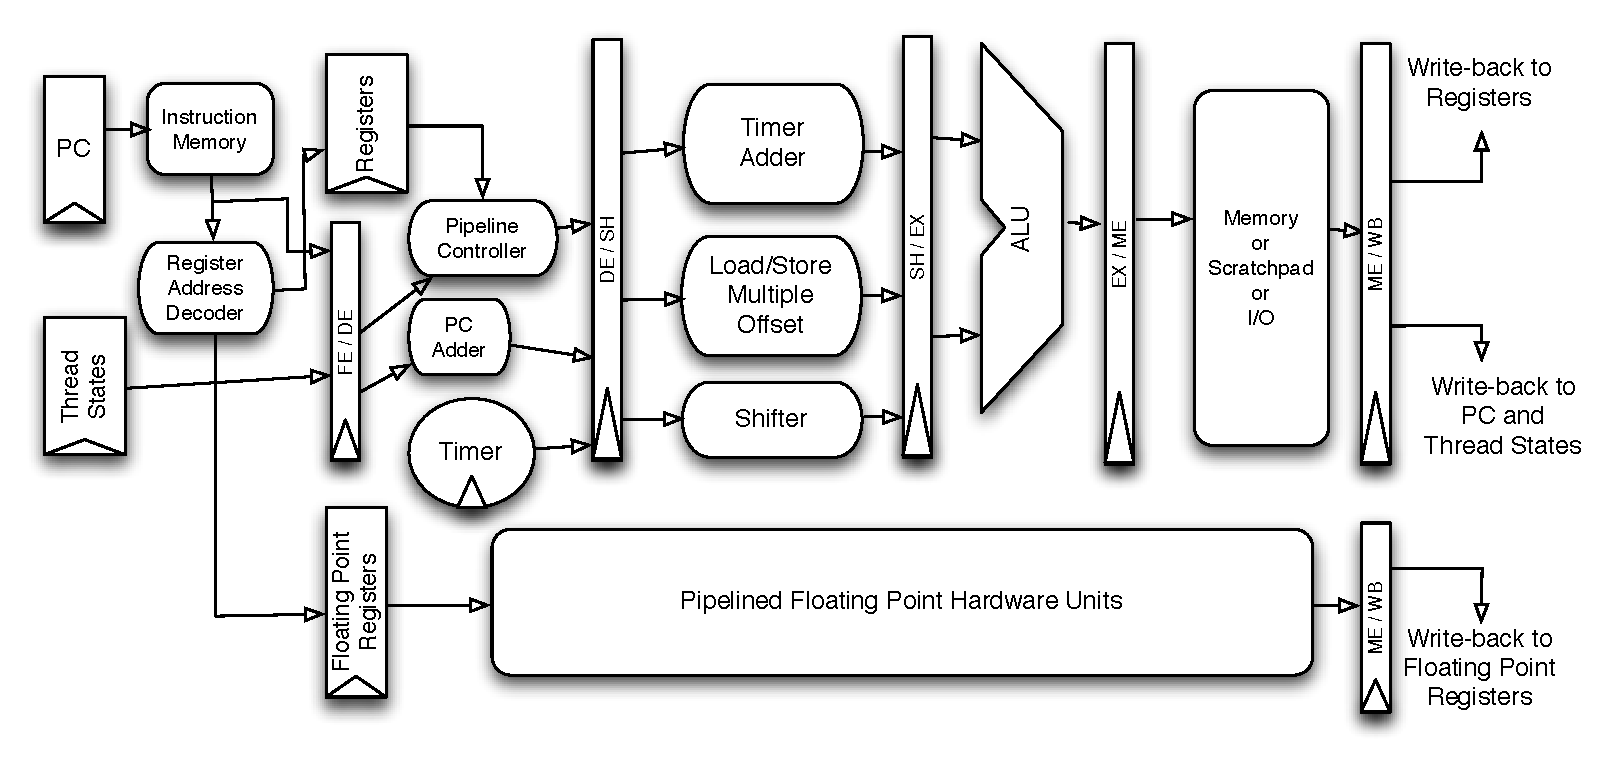
\includegraphics[scale=.6]{figs/ptarm_pipeline_six_stage}
  \end{center}
  \vspace{-20pt}
  \caption{Block Level View of the PTARM 6 stage pipeline}
  \label{fig:ptarm_pipeline_six_stage}
\end{figure}
Here is another header


\begin{figure}
\begin{center}
\vspace{-32pt}

\includegraphics[scale=.45]{figs/placeholder}
\end{center}
\vspace{-12pt}
\caption{Image Placeholder}
\label{fig:placeholder_app}
\end{figure}
